\documentclass{article}
\usepackage[utf8]{inputenc}
\usepackage{placeins}

\usepackage{listings}
\lstset{language=Prolog}
\renewcommand{\lstlistingname}{Código}

\usepackage{amsthm}

\usepackage{qtree}
\usepackage{tikz}



%\theoremstyle{definition}
\newtheorem{definition}{Definição}[section]
\renewcommand\refname{Leituras adicionais}

\theoremstyle{remark}
\newtheorem*{remark}{Remark}

\theoremstyle{theorem}
\newtheorem{theorem}{Teorema}[section]

\usetikzlibrary{shapes.geometric, arrows}
\tikzstyle{decision} = [diamond, minimum width=1cm, minimum height=1cm, text centered, draw=black, fill=green!30]
\tikzstyle{arrow} = [thick,->,>=stealth]

\setlength{\parskip}{.5em}




%
% TODO: revisar esta seção!
%

\begin{document}
\section{Restrições}

Como vimos anteriormente, uma das ideias iniciais da programação lógica era de permitir à programadora expressar \textit{o que} o programa faz, sem ter que se preocupar muito em \textit{como} ele o faz, o que fazemos expressando a lógica do programa em termos de relações. Na maior parte dos paradigmas de programação usuais, há uma dificuldade em expressar essas relações, ou restrições\footnote{Estarmos tratando relação como sinônimo a restrição é um abuso de linguagem usado aqui por sua conveniência, mas é importante lembrar que são coisas diferentes.}, entre os objetos definidos no programa.

Com a programação lógica, isso é um pouco aliviado. Por exemplo, se soubermos a gramática do Prolog, não é difícil ler o programa Member (copiado a seguir, para referência) como expressando uma relação que existe entre um termo X e um Xs se Xs puder ser escrito como {\tt[X|Xz]} ou, se for possível escrever Xs como {\tt [Y|Ys]} e X tiver a relação member com Ys.

\lstinputlisting[caption=Member]{../Exemplos/Cap4/prog1_member.pl}

Mas vimos também que operações aritméticas, no Prolog, não funcionam de maneira relacional (ao fazermos uma soma, por exemplo, o ``+'' funciona como uma função, retornando um valor, no lugar de como uma restrição ou relação). Isso é grave, porque expressões aritméticas aparecem de várias formas em problemas reais e não ser capaz de expressá-las relacionalmente poderia levar a um código muito maior, redundante e difícil de manter.

Para se convencer disso, considere, como um exemplo, a equação da lei de Ohm: I = V/R (onde I é a
corrente, V a tensão e R a resistência).
Claramente, essa equação expressa a relação entre I, V e R, assim como as restrições provenientes dessa relação, indicando que, fixando quaisquer duas das variáveis, a terceira também é fixada e, fixando uma, as duas outras obedecem a uma restrição (por exemplo, se V = 10 volts, temos que $I \times R$ = 10). Atualmente, não conseguimos expressar esse tipo de relação em código sem algum esforço.

Vimos uma forma limitada de lidarmos com isso no capítulo anterior, %TODO Adicionar ref para capítulo
mas precisaremos de algo mais poderoso se quisermos lidar com problemas mais complexos. Antes disso, será útil nos abstrairmos um pouco disso para vermos a programação por restrições de uma forma mais ampla.

\subsection{Domínios}

Restrições não se limita a restrições aritméticas. Existem vários tipos de restrições, cada um possivelmente agindo em diferentes domínos.
O domínio é o que determina as formas legítimas de restrição e o que elas significam. Restrições são escritas usando constantes (como 0, ou 1) e símbolos que agem como funções (como ``+'' ou ``-''). O domínio determina a sintaxe das restrições: quais símbolos de restrições podem ser usados, quais e quantos são os argumentos de cada símbolo e a ordem em que são escritos.

Dois exemplos de domínios que conhecemos são o dos Reais e o dos Inteiros, com os símbolos de restrições usuais (isto é: ``+'', ``$<$'', etc.). Outros exemplos de domínios são o das Árvores e o dos Booleanos. São domínios de grande importância e, por isso, discorriremos momentaneamente um pouco sobre eles logo mais. Em se tratando de domínios aritméticos, a não ser quando dito o contrário, assumiremos que lidamos com o domínio dos Reais.

Definido o domínio, dada uma restrição, precisamos saber o que queremos dela. Algumas das opções mais comuns são:
  \begin{enumerate}
    \item Checar se a restrição é satisfazível (isto é, se existe alguma substituição para o qual a restrição é verdadeira);
    \item Encontrar uma substituição que respeite as restrições;
    \item Otimizar a substituição encontrada por meio de uma função (comumente chamada \textbf{função custo} (apesar de muitas vezes não podermos interpretar essa função como algum ``custo'' de forma natural)\marginpar{\textbf{Função custo}}).
  \end{enumerate}

  Claramente, se conseguimos (2), conseguimos (1) e, se conseguimos (2), conseguimos (1) e (2). Frequentemente, conseguir (1) será equivalente a conseguir (2), porque seguimos um método construtivo. Nem sempre, no entanto, conseguiremos (1). Sabemos, por exemplo, que no domínio dos inteiros existem restrições que não se sabe se podem ser satisfeitas.

  Ou talvez possamos, a princípio, dizer se a restrição em um domínio seja satisfazível, mas na prática isso se torne computacionalmente inviável se a
restrição for muito complicada ou complexa. O problema de descobrir se uma restrição booleana pode ou não ser satisfeita (mais conhecido como SAT, de \textit{Propositional Satisfiability Testing}), é um famoso problema NP-difícil e ainda hoje um tema de ativo pesquisa (veja, por exemplo, \cite{sat}).

Esse tipo de constatação rápida já nos dá uma ideia do tipo de pergunta que precisaríamos fazer dado um domínio, assim como da variedade de tipos de restrição que existem, mesmo em um domínio.

Daqui para frente denotaremos problemas de otimização como COP (de \textit{Constraint Optimization Problem}),  de satisfação de restrições, de CSP (de \textit{Constraint Satisfaction Problem}) e, quando não for necessário fazer distinção, apenas CP. Até agora, temos lidado com CPs como contendo uma restrição, mas será conveniente lidar com eles como contendo uma conjunção de restrições:

Se $x_0$ é um símbolo de restrição no domínio, junto de seus argumentos, diremos que é uma \textbf{restrição primitiva}. Uma \textbf{restrição composta} C é a conjunção de restrições primitivas: $x_0$, ..., $x_n$ (onde as vírgulas, como usual, são lidas como um \textit{e} lógico), onde $x_i$ é uma restrição primitiva. Assim, um COP é descrito por uma tupla (C, f), enquanto que um CSP é descrito por algum C, onde C é uma restrição composta. Daqui para frente nos referiremos a uma
substituição nas variáveis de um CP que respeite às restrições como uma solução desse CP.

\subsection{Árvores}
Como você logo perceberá (ou talvez já o tenha percebido), já vimos restrições por árvores antes, elas só estavam um pouco disfarçadas.

Um \textbf{construtor de árvore} é uma sequência de caracteres começando com uma caractere minúsculo. Definimos uma árvore recursivamente como: uma constante é uma árvore (de altura 1); um construtor de árvore com um conjunto de n $\geq$ 1 árvores é uma árvore.

Árvores são comumente representadas na forma de diagramas como os seguintes:

\Tree[.cons 1 [.cons 2 [.cons 3 4 ] ] ]

ou

\Tree[ .{café da manhã} [.café canela açucar ] {pão de queijo} [.pão queijo ] goiabada ]

Que podem ser reescritos, de forma mais compacta como {\tt cons(1, cons(2, cons(3, 4)))}\footnote{A leitora de olhos afiados vai notar que é mais ou menos assim que representamos listas, trocando o ``cons'' pelo ``.''.} e
{\tt café da manhã(café(canela, açucar), pão de queijo, pão(queijo), goiabada)}\footnote{Estamos usando caracteres especiais aqui para fins de expressividade, mas seu uso em códigos de computador deve ser evitado.}.
Como pode ver, é essencialmente a mesma representação que temos para um funtor (junto com seus argumentos): funtores são árvores, árvores são funtores (neste contexto).

Um algoritmo muito próximo ao algoritmo de unificação, que vimos no Capítulo 1, serve para resolver restrições em árvore do tipo $T_1$ = $T_2$, onde $T_1$ e $T_2$ são árvores. É interessante notar que um algoritmo para resolução de restrições em árvores foi dado por Herbrand\cite{herbrand} de forma independente ao do algoritmo de unificação de Robinson.

Vale notar também outro detalhe importante naquele algoritmo: ele realiza um procedimento que frequentemente fazemos ao buscar resolver um problema, isto é, transformando uma pergunta, potencialmente complicada e difícil, em uma trivial, para o qual sabe-se a resposta. Essa é uma instância de um processo de \textbf{normalização} \marginpar{\textbf{Normalização}}, isto é, um processo de transformar uma restrição em outra equivalente, mas mais tratável. Processos de normalização frequentemente
exercem um papel importante. Voltaremos a esse tema depois.

\subsection{Ideias de resolução}

Nossa discussão sobre problemas envolvendo restrições até agora foi uma discussão geral e apesar de muitas vezes, para resolver esses problemas, ser preferível usar métodos específicos ao domínio e ao tipo de problema, muitas vezes esses problemas são heterogêneos o suficiente para não permitir isso ou não fazem uso de uma sintaxe que permita o uso de métodos específicos.
É útil então termos alguma ou algumas formas gerais de resolver esses problemas. Eles são baseados em busca.

\subsubsection{Propagação local}

Propagação local é melhor explicada por um desenho:

\begin{center}
  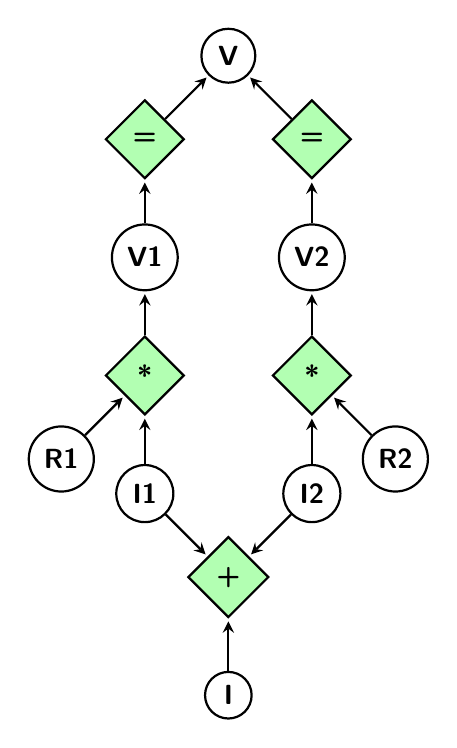
\begin{tikzpicture}[->,>=stealth',shorten >=1pt,auto,node distance=1.5cm, thick,main node/.style={circle,draw,font=\sffamily\bfseries}]

    \node[main node] (V)  {V};
    \node[main node] (eq) [decision, below left of=V]   {=};
    \node[main node] (eq1)[decision, below right of=V]  {=};
    \node[main node] (V1) [below of= eq]                {V1};
    \node[main node] (V2) [below of= eq1]               {V2};
    \node[main node] (tm) [decision, below of=V1]       {*};
    \node[main node] (tm1)[decision, below of=V2]       {*};
    \node[main node] (R1) [below left of=tm]            {R1};
    \node[main node] (R2) [below right of=tm1]          {R2};
    \node[main node] (I1) [below of=tm]                 {I1};
    \node[main node] (I2) [below of=tm1]                {I2};
    \node[main node] (pls)[decision, below right of=I1] {+};
    \node[main node] (I)  [below of=pls]                {I};

    \draw [arrow] (eq) -- (V);
    \draw [arrow] (eq1) -- (V);
    \draw [arrow] (V1) -- (eq);
    \draw [arrow] (V2) -- (eq1);
    \draw [arrow] (R1) -- (tm);
    \draw [arrow] (I1) -- (tm);
    \draw [arrow] (tm) -- (V1);
    \draw [arrow] (tm1) -- (V2);
    \draw [arrow] (I2) -- (tm1);
    \draw [arrow] (R2) -- (tm1);
    \draw [arrow] (I1) -- (pls);
    \draw [arrow] (I2) -- (pls);
    \draw [arrow] (I) -- (pls);

    %\path[every node/.style={font=\sffamily\small}]
      %(1) edge node [left] {0.6} (4)
          %edge [bend right] node[left] {0.3} (2)
          %edge [loop above] node {0.1} (1)
      %(2) edge node [right] {0.4} (1)
          %edge node {0.3} (4)
          %edge [loop left] node {0.4} (2)
          %edge [bend right] node[left] {0.1} (3)
      %(3) edge node [right] {0.8} (2)
          %edge [bend right] node[right] {0.2} (4)
      %(4) edge node [left] {0.2} (3)
          %edge [loop right] node {0.6} (4)
          %edge [bend right] node[right] {0.2} (1);
  \end{tikzpicture}
\end{center}


Esse grafo é uma outra forma de representar a restrição {\tt V=V1, V=V2, V1=I1 $\times$R1, V2=I2$\times$R2, I=I1+I2}\footnote{Exemplo adaptado de \cite{marriot}, pág. 36.}. Considere as restrições adicionais de que {\tt V=8, R1=13, R2=21}. Na propagação local, podemos considerar as arestas como veículos das restrições, deixando-as passar de nó em nó de forma apropriada, passo a passo. Por exemplo, dadas as restrições acima, a restrição de V=8 pode ser propagada para V1=8, e teríamos:


\begin{center}
  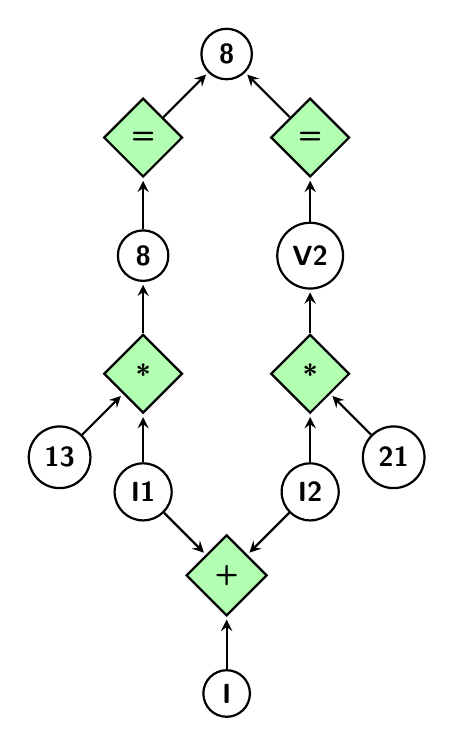
\begin{tikzpicture}[->,>=stealth',shorten >=1pt,auto,node distance=1.5cm, thick,main node/.style={circle,draw,font=\sffamily\bfseries}]

    \node[main node] (V)  {8};
    \node[main node] (eq) [decision, below left of=V]   {=};
    \node[main node] (eq1)[decision, below right of=V]  {=};
    \node[main node] (V1) [below of= eq]                {8};
    \node[main node] (V2) [below of= eq1]               {V2};
    \node[main node] (tm) [decision, below of=V1]       {*};
    \node[main node] (tm1)[decision, below of=V2]       {*};
    \node[main node] (R1) [below left of=tm]            {13};
    \node[main node] (R2) [below right of=tm1]          {21};
    \node[main node] (I1) [below of=tm]                 {I1};
    \node[main node] (I2) [below of=tm1]                {I2};
    \node[main node] (pls)[decision, below right of=I1] {+};
    \node[main node] (I)  [below of=pls]                {I};

    \draw [arrow] (eq) -- (V);
    \draw [arrow] (eq1) -- (V);
    \draw [arrow] (V1) -- (eq);
    \draw [arrow] (V2) -- (eq1);
    \draw [arrow] (R1) -- (tm);
    \draw [arrow] (I1) -- (tm);
    \draw [arrow] (tm) -- (V1);
    \draw [arrow] (tm1) -- (V2);
    \draw [arrow] (I2) -- (tm1);
    \draw [arrow] (R2) -- (tm1);
    \draw [arrow] (I1) -- (pls);
    \draw [arrow] (I2) -- (pls);
    \draw [arrow] (I) -- (pls);

  \end{tikzpicture}
\end{center}

Disso, podemos continuar a propagação, obtendo I1 = 8/13. E assim vai.

Propagação local funciona muito bem para resolver alguns problemas, mas simplesmente não consegue resolver outros. Por exemplo, considere a restrição {\tt A=B+2Z, A=3K-B, K=5, Z=7}. Propagação local detectaria que {\tt K=5} e {\tt Z=7}, mas não encontraria o valor de A ou B. Isso ocorre porque para tanto seria preciso fazer uso de mais de uma restrição por vez, o que a propagação local não faz.

\subsection{Busca Top-Down}

Propagação local pode ser uma técnica muito útil para resolver alguns problemas, e pode ficar mais poderosa ainda se combinada com uma estratégia de \textbf{ramificação}. A essa combinação chamaremos de busca \textit{top-down}.

Intuitivamente, a propagação de restrições ajuda a transformar o problema em outro mais simples. O passo de ramificação serve, então, para partir o problema em problemas menores, aos quais poderemos aplicar a propagação de restrições novamente, seguido por outra ramificação, e assim vai, gerando uma árvore de busca. A forma padrão de busca top-down é chamada de \textbf{busca por \textit{backtracking}}\marginpar{\textbf{Busca por Backtracking}}. Essa forma de busca funciona simplesmente
gerando a dita árvore e fazendo a travessia dela (frequentemente, faremos a travessia enquanto geramos a árvore, não depois). Vale notar que, na presença de propagação de restrições, ocasionalmente pode ser útil adicionar à escrita do problema restrições implícitas, que podem auxiliar na propagação.

A forma mais comum de \textit{backtracking} começa ordenando as variáveis do problema, usualmente por algum modelo heurístico, com as ramificações tomando a forma de divisões no domínio de cada variável. Uma forma de fazer isso é a chamada marcação (ou, mais comumente, \textit{labelling}), que corresponde à ramificação do domínio de cada variável em seus elementos constituintes (o que só pode ser feito, é claro, quando o domínio for finito), assegurando que todos os valores de cada variável
serão explorados. A marcação pode tornar um método de busca incompleto em um completo (isto é, um método que pode não encontrar uma solução quando ela existe em um que sempre encontra alguma solução se ela existe).

A ordem em exploração das variáveis é, então, escolhida por meio de uma \textbf{heurística de escolha de valor}. Frequentemente não será viável termos um método de busca completo, então é essencial que foquemos a nossa atenção nos valores que parecem mais promissores. Esse ``foco de atenção'' pode frequentemente ser descrito na forma de uma política de alocação de crédito, fornecendo maior crédito às escolhas aparentemente mais promissoras.

\subsection{Branch and Bound}

Os métodos de busca discutidos anteriormente são apropriados para CSPs. Para COPs, precisaremos fazer algumas modificações. Uma opção é o \textit{\textbf{branch and bound}}\marginpar{\textbf{Branch and bound}}. Ele funciona da seguinte forma: em cada passo da busca em \textit{backtracking}, se f é a função custo, temos na variável Bound o valor do melhor custo até então (Bound pode ser inicializado com um valor simbólicamente equivalente a ``infinito'') e, a cada passo da busca, checamos
se o custo é ou não melhor do que Bound. Se for, o valor de Bound é atualizado.

Existem algumas variações a esse algoritmo. Uma delas é a de adicionar a restrição de que f $<$ Bound\footnote{Estamos fazendo uso de um abuso de linguagem ao denotar o valor de f em uma substituição por f a fim de deixar a notação mais limpa.}, possibilitando a obtenção de cortes na árvore de busca.

\subsection{Projeção}

Uma ideia implícita em nossa discussão sobre \textit{branch and bound} pode ser vantajosamente generalizada. Considere uma restrição qualquer em função de X, Y e Z, que denotaremos {\tt uma$\_$restrição$\_$qualquer(X, Y, Z)}.

Digamos que só o valor de X nessa restrição seja de interesse. Se tivermos que

{\tt uma$\_$restrição$\_$qualquer(X, Y, Z) :- X > Y, Y > Z, Z > 0.}

\noindenté a única cláusula contribuindo para a definição de {\tt uma$\_$restrição$\_$qualquer(X, Y, Z)}, temos então que X $>$ 0
é a única restrição que nos é de interesse, uma vez que é a restrição de em função de X mais simples que é compatível com a restrição original, no sentido de que a partir de qualquer substituição tal que X $>$ 0 podemos aumentar essa substituição com valores de Y e Z de modo a respeitar a restrição original.

Isso motiva a nossa definição de projeção:

\begin{definition}
  Uma substituição $\iota$ é dita uma solução parcial\marginpar{\textbf{Solução parcial}} de um CP, que chamaremos C, se existe alguma substituição $\rho$ tal que $\iota \cup \rho$ é uma solução de C.
\end{definition}

\begin{definition}
  Dizemos que uma restrição $R_0$ em função das variáveis $X_0$ a $X_n$ é uma projeção\marginpar{\textbf{Projeção}} da restrição $R_1$, em função das variáveis $X_0$ a $X_m$, com m $>$ n, se toda solução de $R_0$ é uma solução parcial de $R_1$.
\end{definition}

Nem todo domínio admite projeções incondicionalmente. O domínio de árvores, por exmeplo, não admite: podemos fazer projeções em algumas restrições nesse domínio, mas não em todas.

O \textit{branch and bound} funciona porque, ao fazer uma ramificação, o que se faz na verdade é uma projeção em uma ou mais variáveis.

Não é difícil ver que a projeção é uma forma de simplificação e, dessa forma, podemos ver o \textit{branch and bound} como uma sequência de simplificações de tipos diferentes.

Simplificações e projeções têm um papel importante na resolução de CPs, então será útil termos uma definição mais rigorosa. Mas antes precisamos da noção de equivalência:

\begin{definition}
  Duas restrições\marginpar{\textbf{Restrições equivalentes}} $C_1$ e $C_2$ são equivalentes em relação ao conjunto de variáveis V, o que denotaremos por $C_1 \leftrightarrow C_2$, se toda solução de $C_1$ restrita a V é uma solução parcial de $C_2$ e se toda solução de $C_2$ restrita a V é uma solução parcial de $C_1$.
\end{definition}

\begin{definition}
  Seja uma restrição composta C, var(X) o conjunto de variáveis de um CP qualquer X e o conjunto de variáveis de interesse inter(C) $\subset$ var(C), dizemos que C' é uma simplificação\marginpar{\textbf{Simplificação}} de C em inter(C) se inter(C) = var(C) e toda solução de C' é uma solução parcial de C.
\end{definition}

É interessante notar que, se dispomos de um algoritmo de simplificação nos moldes dessa definição, também dispomos de um algoritmo de solução: basta simplificar o CP em inter(C) = $\emptyset$.

\subsection{Equivalência}

  Para terminar esta seção, consideremos o problema de equivalência de CPs, o qual é fortemente ligado ao problema de implicação e de bi-implicação. Para tanto, voltamos à questão de normalização:

  \begin{definition}
    Seja \textit{simp} uma função que recebe um CP e um conjunto V de variáveis de interesse e retorna um CP, dizemos que \textit{simp} realiza um processo de \textbf{normalização canônica}\marginpar{\textbf{Normalização canônica}} em um dado domínio se para todo CP C no domínio e todo V $\subset$ var(C), simp(C,V) é uma simplificação de C e se $C_1 \leftrightarrow C_2 \Rightarrow simp(C_1,V) = simp(C_2,V)$.
  \end{definition}

  Com um normalizador canônico, conseguimos responder sem grandes dificuldades a questão de equivalência: dois CPs são equivalentes se a normalização canônica de cada um segundo suas variáveis for idêntica. Daí, também conseguimos saber se um CP implica o outro, ou se o outro implica o um.

  O algoritmo de unificação dado no Capítulo 1 %TODO inserir o ref
é um algoritmo de normalização, como já foi notado, mas não descreve um processo de normalização canônica. Isso ocorre porque não tomamos cuidado suficiente com os nomes das variáveis.

Como poderíamos transformá-lo em um processo de normalização canônica?






  \begin{thebibliography}{1}

    \bibitem{herbrand}
      J. Herbrand (1930), ``Recherches sur la theorie de la demonstration'', PhD thesis, Universite de Paris, France, 1930.

    \bibitem{sat}
      Editores A. Biere, M. Heule, H. Van Maaren, T. Walsh (2009), ``Handbook of Satisfiability'', IOS Press.

    \bibitem{marriot}
      Marriott, Kim; Peter J. Stuckey (1998), ``Programming with constraints: An introduction'' [S.l.]: MIT Press.

  \end{thebibliography}

\end{document}
